\documentclass[12pt, titlepage]{article}

\usepackage{fullpage}
\usepackage[round]{natbib}
\usepackage{multirow}
\usepackage{booktabs}
\usepackage{tabularx}
\usepackage{graphicx}
\usepackage{float}
\usepackage{hyperref}
\usepackage{color}
\hypersetup{
    colorlinks,
    citecolor=black,
    filecolor=black,
    linkcolor=red,
    urlcolor=blue
}
\usepackage[round]{natbib}

\newcounter{acnum}
\newcommand{\actheacnum}{AC\theacnum}
\newcommand{\acref}[1]{AC\ref{#1}}

\newcounter{ucnum}
\newcommand{\uctheucnum}{UC\theucnum}
\newcommand{\uref}[1]{UC\ref{#1}}

\newcounter{mnum}
\newcommand{\mthemnum}{M\themnum}
\newcommand{\mref}[1]{M\ref{#1}}

\title{SE 3XA3: Module Guide\\MovieGuide Application}

\author{Team 35, PGH Software Solutions
		\\ Pratyush Bhandari, bhandarp
		\\ Gazenfar Syed, syedg1
		\\ Hamid Ghasemi, ghasemih
}

\date{\today}



\begin{document}

\maketitle

\pagenumbering{roman}
\tableofcontents

\newpage

\listoftables
\listoffigures

\begin{table}[bp]
\caption{\bf Revision History}
\begin{tabularx}{\textwidth}{p{3cm}p{2cm}X}
\toprule {\bf Date} & {\bf Version} & {\bf Notes}\\
\midrule
Nov 8 & 1.0 & Parts 1 and 2\\
Date 2 & 1.1 & Notes\\
\bottomrule
\end{tabularx}
\end{table}

\pagenumbering{arabic}

 
\newpage
\section{Introduction}

\subsection{Overview}
The MovieGuide project is a re-implementation of an open-source movie reviews Android application which allows users to view ratings, description, and trailers for any movie within the API database.

\subsection{Context}
This is the Module Guide Design Documentation for the MovieGuide re-implementation. Readers of this document include, but are not limited to:

\begin{itemize}
	\item New project members: This document gives an insight into the design structure of the project. It contains information about the module hierarchy along with the modular decomposition, so that new members can quickly learn how each module is integrated into the program.
	\item Maintainers: This document also outlines areas where changes are anticipated which will be helpful to the maintainers as they will be able to quickly identify areas of the application that need to be improved. Moreover, maintainers can utilize the breakdown of the modules to better understand the project structure so that they know which modules to update.
	\item Designers/Developers: This module guide describes the design choices that were made when developing the program. It contains an overview of the relationships between all modules which will aid the designers and developers in determining whether the product design is satisfiable for the software requirements.
\end{itemize}

\subsection{Design Principles}
The design principles utilized for our design choices include information hiding and encapsulation. Information hiding keeps certain aspects of the code a secret from the other modules which reduces the complexity of the program and protects it from extensive modifications that could potentially harm the implementation. Encapsulation combines data and methods allowing internal data to be accessed by public methods. Furthermore, modules were implemented with the principles of high cohesion and low coupling to ensure that the modules are related but not heavily dependent on each other.

\subsection{Document Structure}
This document is organized as specified below:
\begin{itemize}
	\item Section 2: anticipated changes and unlikely changes for the current implementation
	\item Section 3: outlines the module hierarchy 
	\item Section 4: summarizes the relationships between modules and software requirements
	\item Section 5: explains the secret and service/responsibility of each module
	\item Section 6: relates modules to requirements and anticipated changes 
	\item Section 7: describes the uses relations between modules
\end{itemize}

\section{Anticipated and Unlikely Changes} \label{SecChange}
\subsection{Anticipated Changes} \label{SecAchange}
\begin{itemize}
	\item AC1: The API used to retrieve information about movies 
	\item AC2: The format of the input data
	\item AC3: The format of the output data
	\item AC4: The User Interface utilized to navigate through the application
	\item AC5: How movie data is stored locally on the application (ie. improving performance)
\end{itemize}

\subsection{Unlikely Changes} \label{SecUchange}
\begin{itemize}
	\item UC1: The input/output devices (system is designed to run on Android devices) 
	\item UC2: The purpose of the software to provide ratings and descriptions about movies
	\item UC3: The storage method of output data (system assumes there is sufficient storage space on the device, so output data will be stored locally)
\end{itemize}

\section{Module Hierarchy} \label{SecMH}
This section provides an overview of the module design. Modules are summarized
in a hierarchy decomposed by secrets in Table \ref{TblMH}. The modules listed
below, which are leaves in the hierarchy tree, are the modules that will
actually be implemented.

\begin{description}
\item [\refstepcounter{mnum} \mthemnum \label{mHH}:] Hardware-Hiding Module
\item[\refstepcounter{mnum} \mthemnum \label{mHH}:] Input Module
\item[\refstepcounter{mnum} \mthemnum \label{mHH}:] Search Movies Module
\item[\refstepcounter{mnum} \mthemnum \label{mHH}:] Sort Movies Module
\item[\refstepcounter{mnum} \mthemnum \label{mHH}:] Output Module
\item[\refstepcounter{mnum} \mthemnum \label{mHH}:] Searching Algorithm Module
\item[\refstepcounter{mnum} \mthemnum \label{mHH}:] List Object Module
\item[\refstepcounter{mnum} \mthemnum \label{mHH}:] retrofitURL Module
\item[\refstepcounter{mnum} \mthemnum \label{mHH}:] \textcolor{red}{Video Module}
\item[\refstepcounter{mnum} \mthemnum \label{mHH}:] \textcolor{red}{Videoadapter Module}
\item[\refstepcounter{mnum} \mthemnum \label{mHH}:] \textcolor{red}{YoutubeVideos Module}
\item[\refstepcounter{mnum} \mthemnum \label{mHH}:] \textcolor{red}{VideoList Module}

\end{description}


\begin{table}[h!]
\centering
\begin{tabular}{p{0.3\textwidth} p{0.6\textwidth}}
\toprule
\textbf{Level 1} & \textbf{Level 2}\\
\midrule

{Hardware-Hiding Module} & N/A \\
\midrule

\multirow{7}{0.3\textwidth}{Behaviour-Hiding Module} \\
& Input Module\\
& Search Movies Module\\
& Sort Movies Module\\
& Output Module\\

\midrule

\multirow{3}{0.3\textwidth}{Software Decision Module} \\
& Searching Algorithm Module\\
& List Object Module\\
& retrofitURL Module\\
\bottomrule

\end{tabular}
\caption{Module Hierarchy}
\label{TblMH}
\end{table}

\section{Connection Between Requirements and Design} \label{SecConnection}

The design of the system is intended to satisfy the requirements developed in
the SRS. In this stage, the system is decomposed into modules. The connection
between requirements and modules is listed in Table \ref{TblRT} and \ref{TblNRT}. With regards to the main functional requirement of providing a synopsis of every movie, this requirement is fulfilled through the output module, which will provide the service of displaying a specific movie's information when it is clicked on by the user. The searching module, in tandem with the searching algorithm module, will fulfill the functional requirement of having the program list movies based on a specific user query. Lastly, the SortMovies module along with the retrofitURL module will fulfill the functional requirement of allowing the user to sort movies by name, rating or genre.


\section{Module Decomposition} \label{SecMD}

	\subsection{Hardware Hiding Module}
	\textbf{Secret}: The data structure and algorithm used to implement the virtual hardware.\\
	\textbf{Services}:Serves as a virtual hardware used by the rest of the system. This module provides the interface between the hardware and the software. So, the system can use it to display outputs or to accept inputs. \\
	\textbf{Implemented By}: Android OS
	
	\subsection{Behaviour Hiding Module}
	\textbf{Secrets}: The contents of the required behaviours. \\
	\textbf{Services}: Includes programs that provide externally visible behaviour of the system as specified in the software requirements specification (SRS) documents. This module serves as a communication layer between the hardware-hiding module and the software decision module. The programs in this module will need to change if there are changes in the SRS.\\
	\textbf{Implemented By}: MovieGuide \\
	\subsubsection{Input Module}
	\textbf{Secret}:  Inputs \\
	\textbf{Service}: Allows user to scroll, search and click on the list of movies being displayed on the screen.   \\  
	\textbf{Implemented By}: MovieGuide \\
	\subsubsection{Search Movies Module}
	\textbf{Secret}: Search Query\\
	\textbf{Service}: Allows user to enter a search query in the search bar which is then passed as an endpoint to the retrofitURL Module. \\
	\textbf{Implemented By}: MovieGuide\\
	\subsubsection{Sort Movies Module}
	\textbf{Secret}: Movies \\
	\textbf{Service}: Allows user to select different options for sorting the list of movies in the database. \\
	\textbf{Implemented By}: MovieGuide\\ 
	\subsubsection{Output Module}
	\textbf{Secret}: MovieInfoPage \\
	\textbf{Service}: Displays movie information about a specific movie that the user clicked on from the displayed list of movies. \\
	\textbf{Implemented By}: MovieGuide\\
	
	
	\subsection{Software Decision Module}
	\textbf{Secrets}: The design decision based on mathematical theorems, physical facts, or programming considerations. The secrets of this module are \emph{not} described in the SRS. \\
	\textbf{Services}:Includes data structure and algorithms used in the system that do not provide direct interaction with the user. \\
	\textbf{Implemented By}:  -\\
	\subsubsection{Searching Algorithm Module}
	\textbf{Secret}:  Search Algorithm \\
	\textbf{Service}: Uses an algorithm to efficiently find movie matching the search query. \\
	\textbf{Implemented By}: - \\
	\subsubsection{List Object Module}
	\textbf{Secret}: List Object \\
	\textbf{Service}: Stores the list of movies in a ListView object.  \\ 
	\textbf{Implemented By}: -\\
	\subsubsection{retrofitURL Module}
	\textbf{Secret}: API URL \\
	\textbf{Service}: Stores the URL of the API  that GET and POST requests will be sent to. \\ 
	\textbf{Implemented By}: -\\

\section{Traceability Matrix} \label{SecTM}

This section shows two traceability matrices: between the modules and the
requirements and between the modules and the anticipated changes.

% the table should use mref, the requirements should be named, use something
% like fref
\begin{table}[H]
\centering
\begin{tabular}{p{0.2\textwidth} p{0.6\textwidth}}
\toprule
\textbf{Req.} & \textbf{Modules}\\
\midrule
FR1 & M5\\
FR2 & M3,M7,M8\\
FR3 & M3,M7,M5,M8\\
FR4 & M5\\
FR5 & M4,M7\\
\textcolor{red}{FR6} & \textcolor{red}{M9,M10, M11, M12}\\
\bottomrule
\end{tabular}
\caption{Trace Between Functional Requirements and Modules}
\label{TblRT}
\end{table}

\begin{table}[H]
	\centering
	\begin{tabular}{p{0.2\textwidth} p{0.6\textwidth}}
		\toprule
		\textbf{Req.} & \textbf{Modules}\\
		\midrule
		NFR(3.1.1) & M2\\
		NFR(3.1.2) & M2,M5\\
		NFR(3.2.1) & M2\\
		NFR(3.2.3) & M1,M2,\\
		NFR(3.2.4) & M1,M2\\
		NFR(3.2.5) & M2\\
		NFR(3.3.1) & M2,M5\\
		NFR(3.3.2) & M2,M3,M4,M5,M6,M7,M8\\
		NFR(3.3.3) & M2,\\
		NFR(3.3.4) & M1\\
		NFR(3.3.5) & M1, M2, M3, M4, M5, M6, M7, M8\\
		NFR(3.3.6) & M5\\
		NFR(3.3.7) & M3,M4,M6,M7,M8\\
		NFR(3.3.8) & M1,M2,M3,M4,M5,M6,M7,M8\\
		NFR(3.4.1) & M1\\
		NFR(3.4.2) & M1,M2,M3,M4,M5,M6,M7,M8\\
		NFR(3.4.3) & M2,M5\\
		NFR(3.4.4) & M2,M3,M4,M5,M6,M7,M8\\
		NFR(3.5) & M2,M3,M4,M5,M6,M7,M8\\
		NFR(3.6.1) & M3,M4,M6,M7,M8\\
		NFR(3.6.2) & M3,M4,M6,M7,M8\\
		NFR(3.6.3) & M2,M3,M4,M6,M7,M8\\
		NFR(3.6.5) & M3,M4,M6,M7,M8\\
		NFR(3.7) & M5\\
		NFR(3.8) & M1,M3,M4,M5,M6,M7,M8\\
		\bottomrule
	\end{tabular}
	\caption{Trace Between Non-Functional Requirements and Modules}
	\label{TblNRT}
\end{table}


\begin{table}[H]
\centering
\begin{tabular}{p{0.2\textwidth} p{0.6\textwidth}}
\toprule
\textbf{AC} & \textbf{Modules}\\
\midrule
AC1 & M8\\
AC2 & M2\\
AC3 & M5\\
AC4 & M2,M5,M7\\
AC5 & M5\\

\bottomrule
\end{tabular}
\caption{Trace Between Anticipated Changes and Modules}
\label{TblACT}
\end{table}



\section{Use Hierarchy Between Modules} \label{SecUse}

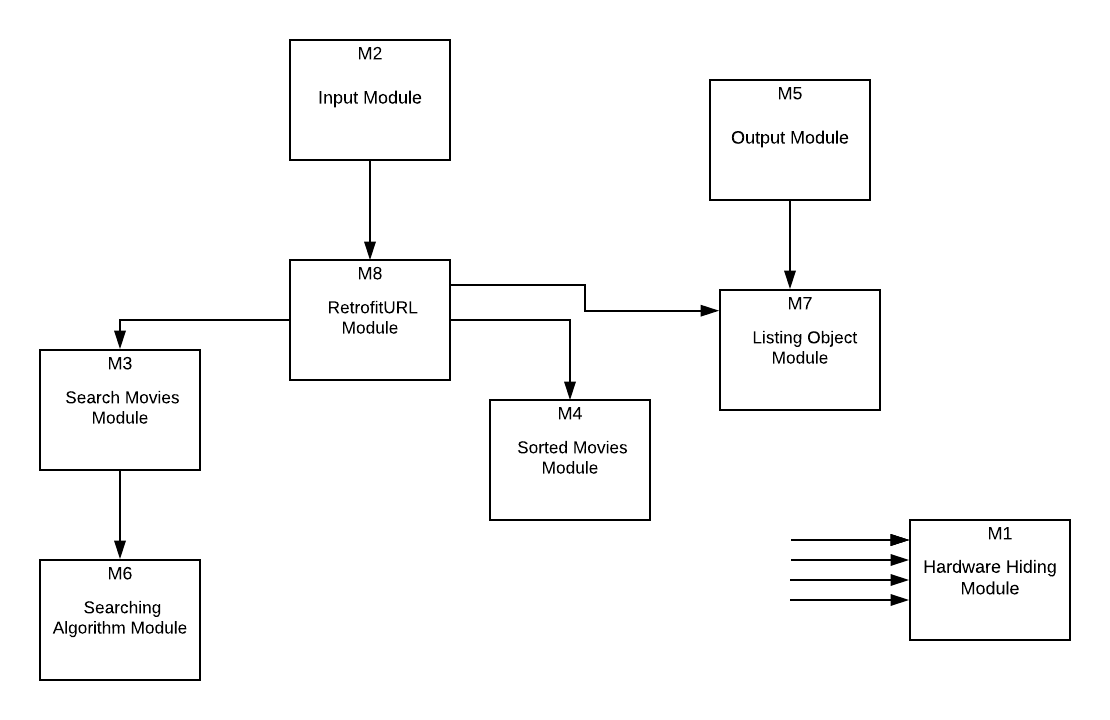
\includegraphics{3}

\begin{figure}[H]
\centering
%\includegraphics[width=0.7\textwidth]{UsesHierarchy.png}
\caption{Use hierarchy among modules}
\label{FigUH}
\end{figure}

\end{document}